\chapter{Definitions}

In this chapter, we will cover the basic definitions and concepts related to complex networks. We will start with fundamental graph concepts, then explore various network representations, discuss graph isomorphism and permutation, and finally delve into connectedness, distances, subgraphs, planarity, homomorphism, network reduction, and spectral analysis of networks.

\section{Basic Graph Concepts}

\begin{definition}[Graph]
    A graph $G(V,L)$ is a finite nonempty set $V$ of $p$ points (vertexes or nodes) and a set of $k$ couples of distinct points $L$ (links, lines, or edges).
\end{definition}

\begin{remark}[General Rules]
    \begin{itemize}
        \item In general, networks have no loops (self-connections).
        \item There are no multigraphs, meaning no multiple links between the same nodes.
        \item We can, however, consider multiple links as weights or as multiple layers (multiplex).
    \end{itemize}
\end{remark}

\subsection{Directed and Undirected Graphs}
Directed graphs (DiGraphs) are graphs with directed edges, known as arcs, indicating a ``from-to'' relationship. They are used to describe hierarchical relationships, fluxes, or the passing of messages and goods. Undirected graphs contain only symmetric links and are used to describe symmetrical relations such as friendship, chemical bonds, or statistical correlation. Note that directed graphs can be symmetrized; while this loses some information, it allows the use of simpler properties and algorithms.

\subsection{Walk, Trail, Path, and Cycle}

Let us consider a graph with nodes $i$ and $j$. We can define different types of connections between these nodes:
\begin{itemize}
    \item \textbf{Walk}: A node and edge sequence between two nodes.
    \item \textbf{Trail}: A walk with all distinct links.
    \item \textbf{Path}: A walk with all distinct nodes and links.
    \item \textbf{Cycle}: A closed path with $N_c \ge 3$ nodes.
\end{itemize}
This classification is important for understanding the structure of networks and for defining concepts such as connectedness and distances. Different algorithms are used to find walks, trails, paths, and cycles in a graph, which can be crucial for applications like network traversal, routing, and community detection.

\section{Network Representations}

It is important to note that a graph can be represented in various ways, each with its own advantages and disadvantages. The choice of representation often depends on the specific application and the properties of the graph being studied.

\subsection{Adjacency Matrix}

The most common representation of a graph is the adjacency matrix, which is a square matrix that encodes the presence or absence of links between nodes. For unweighted graphs, the entries are binary (0 or 1), while for weighted graphs, the entries can take on a range of values corresponding to the weights of the links.

\begin{definition}[Adjacency Matrix]
    The adjacency matrix $A$ is an $N \times N$ matrix representing $N$ nodes. For unweighted networks, $A_{ij}=1$ indicates a topological link from node $i$ to node $j$, with $A_{ii}=0$ to indicate no loops. For weighted networks, $A_{ij}=w_{ij}$ where $w_{ij}$ is the weight of the link.
\end{definition}

\begin{minipage}{0.45\textwidth}
    \textbf{Directed Graph}

    Consider the following directed graph with 6 nodes, we can represent it with the following adjacency matrix:
    \begin{figure}[H]
        \centering
        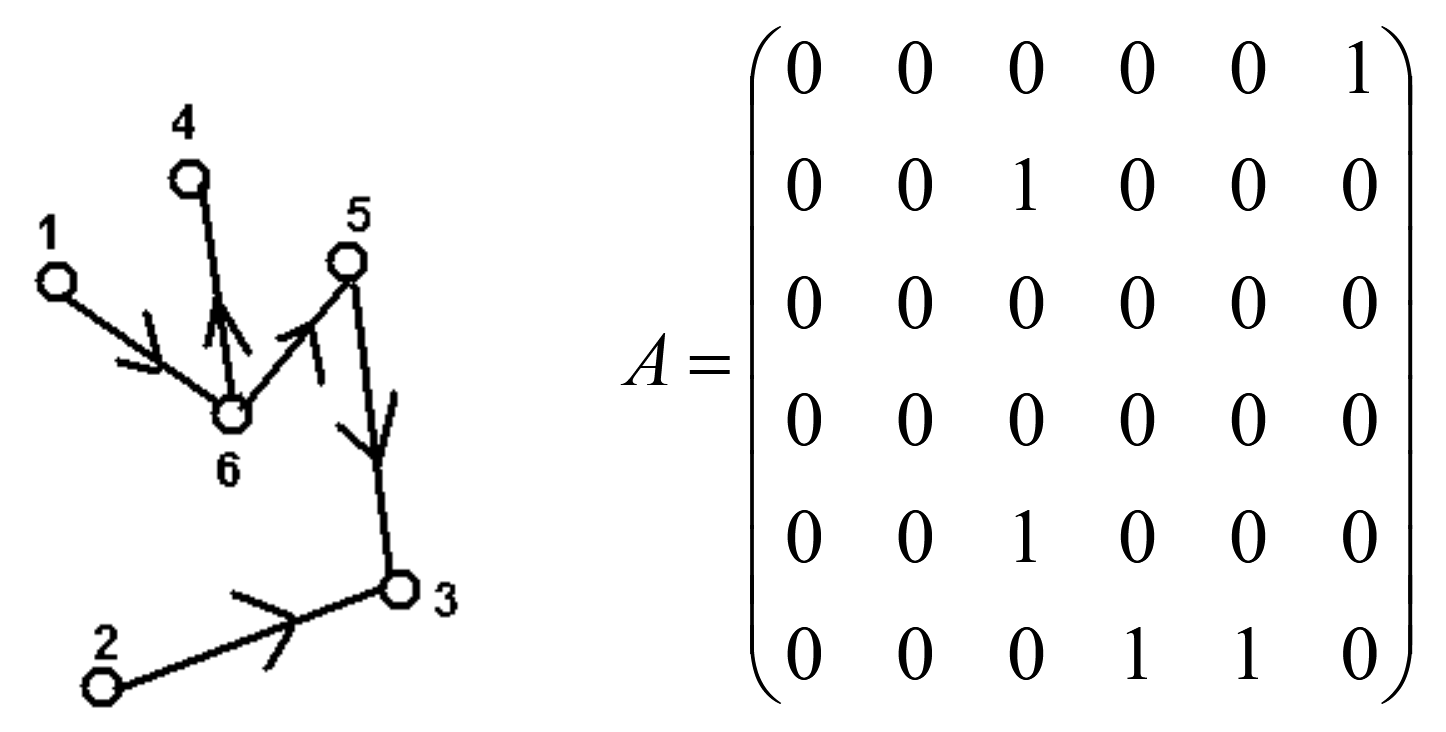
\includegraphics[width=\textwidth]{img/generic_adjacency.png}
        \caption{A directed graph and its corresponding non-symmetric adjacency matrix.}
    \end{figure}
\end{minipage}
\hfill
\begin{minipage}{0.45\textwidth}
    \textbf{Undirected Graph}

    Consider the following undirected graph with 6 nodes, we can represent it with the following adjacency matrix:
    \begin{figure}[H]
        \centering
        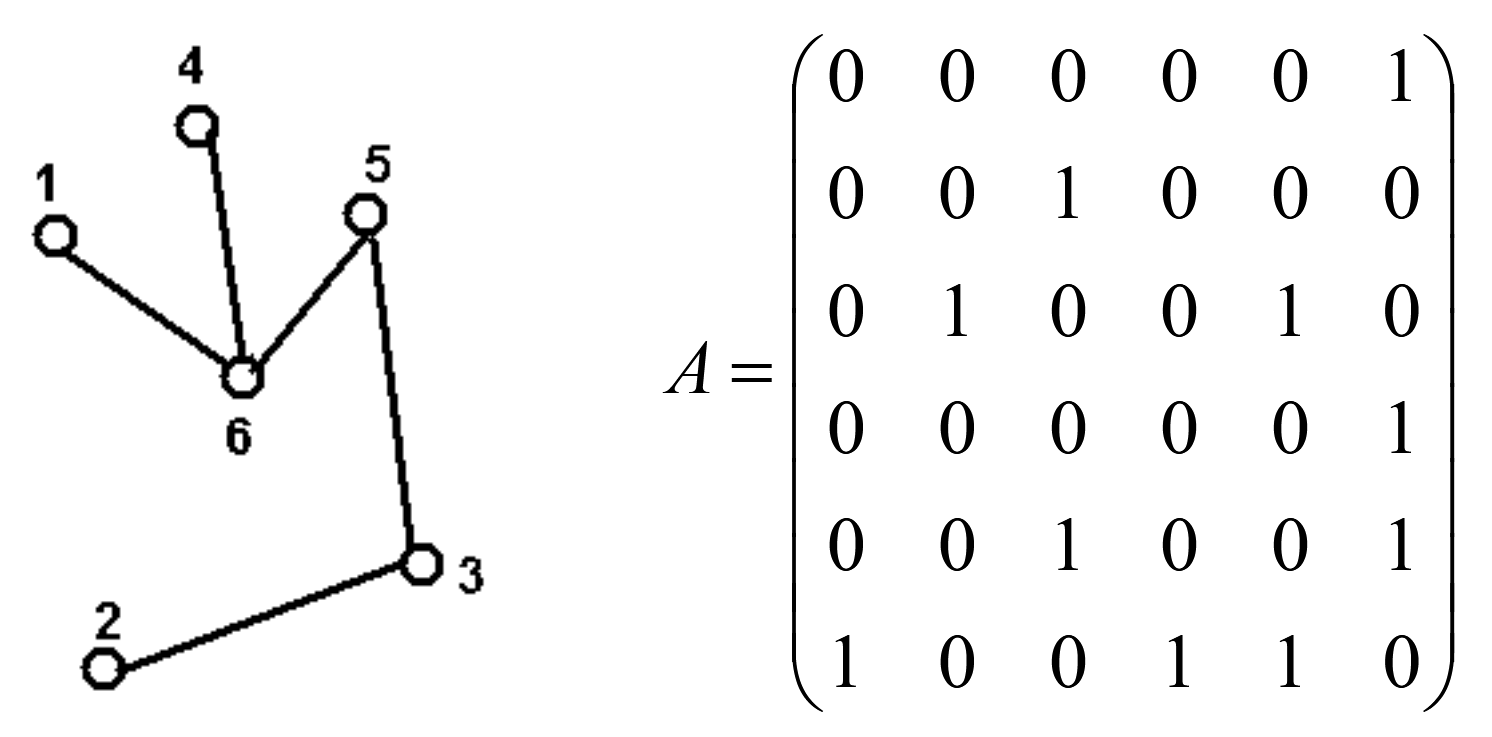
\includegraphics[width=\textwidth]{img/symmetric_adjacency.png}
        \caption{An undirected graph and its corresponding symmetric adjacency matrix.}
    \end{figure}
\end{minipage}

\begin{remark}[Logical Operators on Adjacency Matrices]
    We can apply element-wise logical operators on adjacency matrices:
    \begin{itemize}
        \item Network symmetrization uses a logical OR: $A' = \max(A, A^T) = A \cup A^T$.
        \item Identifying reciprocal links uses a logical AND: $A'' = \min(A, A^T) = A \cap A^T$.
        \item Identifying strictly directed links uses logical XOR: $XOR(A, A^T)$.
    \end{itemize}
\end{remark}

\subsection{Weighted Network}

In a weighted network, the adjacency matrix contains values that represent the strength of the connections between nodes:
\[
    A_{ij} = w_{ij} \text{ link from node } i \text{ to node } j \text{ with weight } w_{ij}.
\]
This can be interpreted in various ways depending on the context, such as the number of interactions, the intensity of relationships, or the capacity of links.

It can be seen as a representation of a \textbf{multigraph} with N multi-edges: \(w_{ij} = N\). If all weights are positive, we have useful theorems for matrices with positive values (Perron-Frobenius theorem) and we can connect to "physical" situations (transition probabilities of diffusion processes)
Negative weights can be meaningful too: in \textbf{signed networks} the sign of the weight can represent different types of relationships or interactions, such as:
\begin{itemize}
    \item \textbf{Friend-enemy}: in social networks, positive weights can represent friendships while negative weights can represent enmity.
    \item \textbf{Attraction-repulsion}: in physical systems, positive weights can represent attractive forces while negative weights can represent repulsive forces.
    \item \textbf{Ferromagnetic-antiferromagnetic}: in spin systems, positive weights can represent ferromagnetic interactions while negative weights can represent antiferromagnetic interactions.
\end{itemize}

One can also operate a weighted matrix symmetrization:
\begin{itemize}
    \item Average symmetrization: $A' = \frac{1}{2}(A + A^T)$.
    \item Random matrix symmetrization: $A' = \frac{1}{\sqrt{2}}(A + A^T)$.
\end{itemize}

\subsection{Incidence Matrix}

We can also represent a graph using an incidence matrix, which is an alternative to the adjacency matrix. The incidence matrix is particularly useful for certain types of analyses, such as flow problems and network dynamics.

\begin{definition}[Incidence Matrix]
    The incidence matrix $I$ of a graph $G(V,L)$ is an $L \times V$ matrix (number of links by number of vertexes). It contains $-1$ for outgoing connections and $+1$ for ingoing connections:
    \[
        \text{if } A_{ij} \neq 0, \quad I_{Ni} = \mp 1, \quad I_{Nj} = \pm 1.
    \]
    It can be interpreted as a ``generalized derivative'' on the graph, giving the oriented difference between values on adjacent nodes.
\end{definition}

Thus the incidence matrix can be used to analyze the flow of information or resources through the network, and it is particularly useful for studying directed graphs and their properties. The incidence matrix can also be used to derive the adjacency matrix through the relation $A = I^T I - D$, where $D$ is a diagonal matrix that accounts for the degree of each node.

\subsubsection{Generalized Derivative}

The incidence matrix can be interpreted as a generalized derivative on the graph, giving the oriented difference between values on adjacent nodes. The incidence matrix allows us to compute the net flow into or out of each node, which is essential for understanding the dynamics of processes.

Given a vector of values \(\mathbf{f}_i\) for each node, the incidence matrix \(I\) applied on the vector gives:
\[
    \begin{aligned}
        \sum_{j} I_{ij} \cdot \mathbf{f}_j & = \Delta_i,                                                  \\
        \Delta_i                           & = \mathbf{f}_i - \mathbf{f}_j \forall \text{adjacent nodes},
    \end{aligned}
\]
where \(\Delta_i\) represents the net flow into or out of node \(i\) based on the values of its neighbors. This interpretation is crucial for analyzing diffusion processes, random walks, and other dynamic phenomena on networks.

Geometrically, a network acts as a spatial structure: while a regular lattice discretizes Euclidean space, a complex graph represents a more intricate manifold. However, one must be careful, as the properties of this discrete manifold do not necessarily hold in the continuous limit.

\subsection{Sparse Representations}
For sparse graphs where the number of links is much smaller than $V^2$, other representations are preferred:
\begin{itemize}
    \item \textbf{Edge Matrix}: An $L \times 2$ matrix that stores single links instead of the full matrix.
    \item \textbf{Adjacency List}: Each line describes a node and contains the indices of its arrival nodes. This is particularly useful for diffusion processes, such as simulating random walks on a graph.
\end{itemize}

% --------------------------------------------------------
\section{Graph Isomorphism and Permutation}
% --------------------------------------------------------

\begin{definition}[Graph Isomorphism]
    An isomorphism is a 1-1 correspondence between vertexes that preserves the link structure. It corresponds to a node index permutation.
\end{definition}

\begin{remark}[Re-indexing]
    Node permutation represents node reordering. Re-indexing can be based on a priori information (like intrinsic metrics) or network-based centrality measures, and is very important for network visualization.
\end{remark}

\begin{example}[Protein and DNA Contact Maps]
    A network representation of peptide bonds serves as a discretization of a 3D distance matrix. Spatial closeness acts as an ``intrinsic'' metric for the graph.
\end{example}

% --------------------------------------------------------
\section{Connectedness}
% --------------------------------------------------------

\subsection{Undirected Graphs}
An undirected graph is connected if it is not divided into two or more non-communicating parts. Algebraically, this means there is no permutation that reduces the adjacency matrix into diagonal blocks.

\subsection{Directed Graphs}
In a directed graph, not every node is necessarily reachable from any other. Connectedness is classified into three types:
\begin{itemize}
    \item \textbf{Strongly connected}: Every node is connected to another by a path, implying the existence of cycles.
    \item \textbf{Unilaterally connected}: For every two nodes, there is at least one path.
    \item \textbf{Weakly connected}: Every node is connected to another by at least a semipath.
\end{itemize}

\begin{remark}[Block Matrix Reduction]
    For directed graphs, the adjacency matrix can sometimes be reduced to blocks where nodes in block C are reachable from block A, but not vice versa. In such cases, block C acts like a ``sink'' or ``absorbing state'' in transition processes.
\end{remark}

% --------------------------------------------------------
\section{Distances and Shortest Paths}
% --------------------------------------------------------

\subsection{Node Distance}
The distance between two nodes is defined as the shortest path between them. In weighted networks, nodes that are ``closer'' have a greater weight, and distance can be calculated using harmonic composition (similar to capacitors in series). The larger the weight, the smaller the distance.

\subsection{Shortest Path Algorithms}
The distance between two nodes equals the minimum number of links (geodesic) between them. The diameter of a graph is the maximum path length, while the average path length is the average over all paths. These are typically calculated using Dijkstra's algorithm (one-to-all) or the Floyd-Warshall algorithm (all-to-all).

% --------------------------------------------------------
\section{Subgraphs and Special Network Topologies}
% --------------------------------------------------------

\subsection{Subgraphs and Cliques}
\begin{definition}[Induced Subgraph e K-Clique]
    \begin{itemize}
        \item \textbf{Subgraph}: A subset of a graph's nodes and links.
        \item \textbf{Induced Subgraph}: A subset of the nodes of $G$ with ALL the links of $G$ that exist between those specific nodes.
        \item \textbf{K-Clique}: A fully connected subgraph with degree $K$.
    \end{itemize}
\end{definition}

\subsection{Complete Graphs}
A completely connected graph $K_N$ has all possible links, meaning every node has a degree of $K = N-1$. The graph complement has the same nodes but the ``opposite'' links.

\subsection{Bipartite Graphs}
\begin{definition}[Bipartite Graph]
    A graph that connects two different types of nodes between each other, but NOT between themselves. It is represented by an $M \times N$ rectangular adjacency matrix. In terms of matrix algebra, a bipartite graph is an imprimitive matrix of order 2.
\end{definition}

\begin{remark}[Tensor Contraction]
    Given a rectangular adjacency matrix $B$ representing a bipartite graph, we can obtain two square networks connecting nodes of the same type via contraction: $B \cdot B^T$ and $B^T \cdot B$. Nodes of the same type are connected if there is at least one path between them through a node of the other type.
\end{remark}

\begin{example}[The Human Disease Network]
    An example of a bipartite graph is the ``diseasome'' (e.g., OMIM database), a gene-pathology network. By contracting the matrix, we can obtain a gene-gene network based on shared diseases, or a pathology-pathology network based on shared genes.
\end{example}

\subsection{Trees, Stars, and DAGs}
% Star Network, Trees (forest, fractals) e Directed Acyclic Graphs (DAG)[cite: 1212, 1216, 1221, 1229, 1230].

\begin{remark}[DAG Adjacency Matrix]
    % Matrice triangolare superiore, nilpotent matrix[cite: 1274, 1275, 1276].
\end{remark}

% --------------------------------------------------------
\section{Planarity and Homomorphism}
% --------------------------------------------------------

\subsection{Planarity and Genus}
% Teorema di Kuratowski (K5, K3,3) e limiti dei link[cite: 1187, 1188, 1191, 1192].

\subsection{Graph Homomorphism}
% Dimensionality reduction mantenendo l'adiacenza[cite: 1194, 1195, 1197].

% --------------------------------------------------------
\section{Network Reduction and Filtering}
% --------------------------------------------------------

\subsection{Minimum Spanning Tree (MST)}
\begin{definition}[Min/Max Spanning Tree]
    % Riduzione della rete a un tree backbone[cite: 1280, 1281].
\end{definition}
% Algoritmi di Kruskal e Prim[cite: 1287, 1293].

\subsection{Link Selection Rules}
% Global thresholding vs Local rule (es. Serrano et al.)[cite: 1307, 1309, 1312, 1314].

% --------------------------------------------------------
\section{Spectral Analysis of Networks}
% --------------------------------------------------------

\subsection{The Eigenvalue Spectrum}
% Eigenvalue problem e characteristic polynomial[cite: 1399, 1401, 1403].

\subsection{Powers of the Adjacency Matrix}
% Interpretazione di A^k come numero di walks di lunghezza k[cite: 1406, 1413, 1414].

\subsection{Spectra of Specific Graphs}
% Spettri per Directed cycles, Completely connected graphs, Bipartite graphs e DAG[cite: 1418, 1424, 1435, 1441].

\subsection{Isomorphism and Co-spectrality}
\begin{remark}[Co-spectrality]
    % Isomorphic implica cospectral, ma non viceversa[cite: 1461, 1463].
\end{remark}

\subsection{Graph Distances}
% Graph spectral distance e Graph edit distance[cite: 1509, 1516].